%
%  untitled
%
%  Created by vbosch on 2011-02-07.
%  Copyright (c) 2011 McBosch. All rights reserved.
%
\documentclass[a4paper,10pt,titlepage]{article}

% Use utf-8 encoding for foreign characters
\usepackage[utf8]{inputenc}

% Setup for fullpage use
\usepackage{fullpage}
\usepackage{titlepic}
\usepackage{float}
\usepackage{color}

% Uncomment some of the following if you use the features
%
% Running Headers and footers
%\usepackage{fancyhdr}

% Multipart figures
%\usepackage{subfigure}

% More symbols
\usepackage{amsmath}
%\usepackage{amssymb}
%\usepackage{latexsym}

% Surround parts of graphics with box
\usepackage{boxedminipage}

% Package for including code in the document
\usepackage{listings}

% If you want to generate a toc for each chapter (use with book)
\usepackage{minitoc}

% This is now the recommended way for checking for PDFLaTeX:
\usepackage{ifpdf}

%\newif\ifpdf
%\ifx\pdfoutput\undefined
%\pdffalse % we are not running PDFLaTeX
%\else
%\pdfoutput=1 % we are running PDFLaTeX
%\pdftrue
%\fi

\ifpdf
\usepackage[pdftex]{graphicx}
\else
\usepackage{graphicx}
\fi
\title{Neural Networks \\ Course Project - Terrain Classification}
\author{Vicente Bosch Campos \dag \\
\textcolor{blue}{\texttt{viboscam@posgrado.upv.es}}}
\titlepic{\includegraphics[width=250pt]{cover.jpg}}

\date{\today}

\begin{document}

\ifpdf
\DeclareGraphicsExtensions{.pdf, .jpg, .tif}
\else
\DeclareGraphicsExtensions{.eps, .jpg}
\fi

\maketitle

\tableofcontents

\listoffigures

\section{Introduction}

\par The application of Multilayer Perceptron and Support Vector Machines to uni - dimensionally multi-spectral representation of a 3x3 pixel matrix of an image section to recognize terrain type of the central pixel is considered in this course project.
\\
\par The use of Pattern Recognition and Image Analysis is quite established for the task of satellite image classification. In this course project we consider the classification of terrain types.


\subsection{Data}


\par A Landsat MSS image consists of four digital images of the same zone using different spectral bands. Two of the bands are in the visible region (corresponding approximately to green and red regions of the visible spectrum) while the other two are in the (near) infra-red. Each pixel is represented as a 8-bit binary word, with 0 corresponding to black and 255 to white. The spatial resolution of a pixel is approximately 80m x 80m. Each image contains 2340 x 3380 such pixels.
\\
\par The database used in the course project is a sub-area of a scene, consisting of 82 x 100 pixels. Each line of data corresponds to a 3x3 square neighborhood of pixels completely contained within the 82x100 sub-area. Each line contains the pixel values in the four spectral bands (converted to ASCII) of each of the 9 pixels in the 3x3 neighborhood and a number indicating the classification label of the central pixel. As per the original database the number is a code for the following classes:
\begin{enumerate}
	\item red soil
	\item cotton crop
	\item grey soil
	\item damp grey soil
	\item soil with vegetation stubble
	\item mixture class ( all types present)
	\item very damp grey soil
\end{enumerate}



\par Further preprocessing has been performed to the data provided to us. It has been normalized and as there are no records of the 6th type the classes label have been moved so that type 7 is represented by the label 6. 

\par We have been provided with two data partitions:
\begin{itemize}
	\item sat6c.tra.norm: Training set formed by 2000 records with the following composition:
	\begin{itemize}
		\item Class 1: 471
		\item Class 2: 220
		\item Class 3: 440
		\item Class 4: 197
		\item Class 5: 213
		\item Class 6: 459
	\end{itemize}
	\item sat6c.public.tst.norm: Public test set containing of 1000 records with the following composition: 
	\begin{itemize}
		\item Class 1: 241
		\item Class 2: 92
		\item Class 3: 210
		\item Class 4: 96
		\item Class 5: 106
		\item Class 6: 255
	\end{itemize}
\end{itemize}


\subsection{Scope}

\par As part of the course project we will train classifiers for the landstat task described in the above sections. To be more precise we will use the following techniques:
\begin{itemize}
	\item Multilayer Perceptron:
		\begin{itemize}
			\item Back propagation with momentum
			\item Quick propagation
			\item Radial Networks
		\end{itemize}
\end{itemize}

\par In order to evaluate the classifiers trained they will be sent to an external oracle containing a private data set in order to determine the test error with an independent data set.  

\section{Development}

\par In this section we will describe the software framework developed in order to perform the experimentations for the task. The framework developed allows us to load, format and perform transformations with specific data sets and also launch classifier training with different classifiers and obtain mean test set classification error with cross validation. 

\subsection{Software Structure}

\par The software is structured into the following classes:
\begin{description}
	\item[DataPattern:] The DataPattern class is defined in the \textit{./lib/data\_pattern.rb} file. It encapsulates a sample record of class containing the actual data ( can be in numeric or string representations) and the class label. It allows us to perform the following operations: 
	\begin{itemize}
		\item Order to records by label value.
		\item Iterate over the different values of the vector.
		\item Duplicate the record.
	\end{itemize}
	\item[DataSet:] The DataSet class can be found in the \textit{./lib/data\_set.rb} file. It represents a whole set of records of a task allowing us to perform the following tasks over them:
	\begin{itemize}
		\item Read the original data from a file and apply specific format to them to prepare them for the ML tool. e.g. Uniform the chain length for a Chromosome classification task. 
		\item Write them to file using an specific format for a ML toolset.
		\item Partition the set into blocks ensuring correct representation and number of each class in the block.
		\item Combine different sets in an additive manner.
		\item Sort the set by class label.
	\end{itemize}
	\item[Snns:] The Snns class can be found in the \textit{./lib/snns.rb} file. It is an object wrapper for the Batchman snns interface and allows us to perform the following tasks from the framework:
	\begin{itemize}
		\item The class allows as input an experiment object, it automatically generates an specific batchman script file and runs it. 
		\item Permits us to programmatically access to the results of the .res files when reviewed with the analyze tool.
	\end{itemize}
	\item[SnnsFileWriter:] The SnnsFileWriter class can be found in the \textit{./lib/snns.rb} file. The file writer is in charge of performing header and footer special formatting for the toolset chosen. In this case it allows us to call mkhead from the framework to prepare the pattern files. 
	\item[SnnsPatternWriter:] It can be found in \textit{./lib/snns.rb}. The pattern writer in in charge of performing special formatting to the patterns required for correct usage on the desired toolset. In this case it ensures there is a space between each dimension value and ensures there is a line space between the vector and the class label. 
	\item[Parameter:] Coded in \textit{./lib/parameter.rb}. The class allows us to define a parameter and a range of values of variation. The values can be a set of strings, if for example we want to vary between different neural network files or a numeric value, to study an specific range of the momentum parameter. 
	\item[Experiment:] Present in the file \textit{./lib/experiment.rb}. It is an specific configuration, value set, of the parameters that will be executed on the chosen ML tool set and the value will be averaged over cross experimentation. 
	\item[Study:] contained in \textit{./lib/study.rb}. It generates the set of experiments by performing combinations of each of the values for each parameter described and runs them writing the results and studies performed in specific files. 
\end{description}
\subsection{Library Options}

\par With the defined software structure we can easily perform studies on an indicated task by just having to write the specific
read and write formatters for the task. Next we will show a short example of the framework scripts used to train neural networks 
for the chromosome classification task: 

\lstset{basicstyle=\footnotesize,language=Ruby}
\lstset{linewidth=500pt}
\lstset{numbers=left, stepnumber=1}
\lstset{commentstyle=\color{blue}, stringstyle=\color{green},showspaces=false}
\lstset{keywordstyle=\color{red}\bfseries\emph}
\lstset{frame=trBL,frameround=tttt}
\lstinputlisting[caption=chromosome.rb,label=lst:lowertri]{./bin/rn_practice.rb}

\subsection{Software Output}

\par The software generates the following output files that will help us out for the review of the classification training:

\begin{description}
	\item[Study List:] Is a detailed print out indicating the parameters used in the experiment as well as the pattern files and output files in case the experiment wants to be reviewed in detail:
	{\footnotesize\begin{verbatim}
______________________________________________________________________________________
1
{:algo=>"Quickprop", :in_model=>"../test/theory_data/trr_36_20_6.net", :learning=>0.15000000000000002, :max_growth=>0.1, 
:id=>1, :test_pat=>"./QP30_20_6/20110209-000607_test.pat", :val_pat=>"./QP30_20_6/20110209-000607_val.pat", 
:train_pat=>"./QP30_20_6/20110209-000607_train.pat", :out_model=>"./QP30_20_6/20110209-000607Quickprop.net", 
:test_res=>"./QP30_20_6/20110209-000607test.res", :val_res=>"./QP30_20_6/20110209-000607val.res"}
______________________________________________________________________________________
	\end{verbatim}}
	
	\item[Result File:] For each of the parameter combinations a result is printed out containing the mean error, wrong and right classification \% for the validation and test set over the cross training.
	\item[Log files:] Contains an execution log of the Batchman execution with the training and validation MSE.
	\item[Bat files:] Automatically generated Batchman script for the experiment.
	\item[Snns standard files:] It also generates and saves the following SNNS files:
	\begin{itemize}
		\item Result files of the validation and test sets.
		\item Pattern files used in the training.
		\item Resulting neural network.
	\end{itemize}
\end{description}


\section{Experimental Results}
\subsection{Neural Networks}

\par For the Neural Networks experiments a cross validation over 10 blocks will be performed for each experiment. The data will be composed of the training plus the public data set given.

\par Once selected the best result of an specific range/parameter/topology study the parameters are repeated in a 30 block cross validation sending one of the trained networks sent to the oracle to obtain private test data set classification result.

\subsubsection{Back Propagation with Momentum}

\par As it is dependent of the task all networks tested where configured with 36 input neurons and 6 output neurons connected in feed forward with out shortcuts. For the selection of the best hidden layer configuration, the following where tested:
\begin{itemize}
	\item One hidden layer: 15,20,30,40,50,60,70,80,90 and 100 neurons.
	\item Two hidden layers: 10-10 neurons in each layer. 
\end{itemize}

\par For each topology a study was launched varying the learning factor from 0.1 to 0.6 in increments of 0.05 and for each learning factor value the momentum was varied from 0.1 to 0.5 in 0.1 increments. Hence for each topology 55 different training set factors where tested, considering the 10 block cross validation and the 11 different topologies: 6050 networks where trained. 

\par Next we will show a set of graphics to summarize the results obtained: 


\begin{figure}[H]
	\centerline{%
	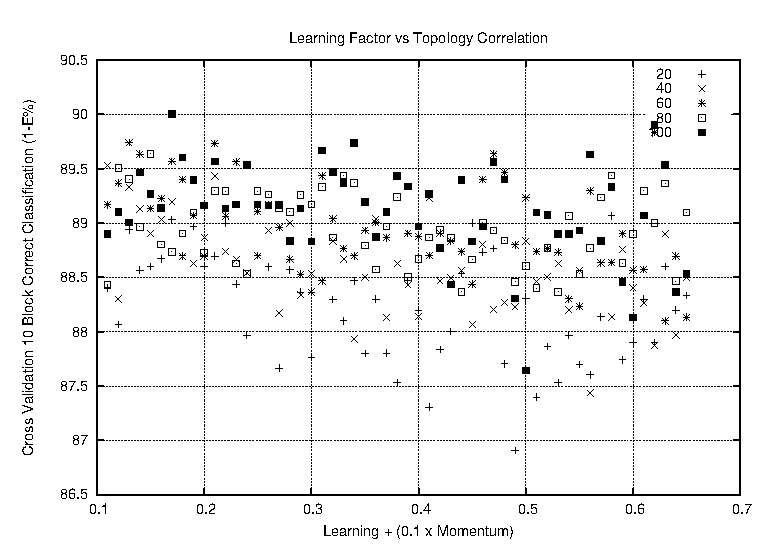
\includegraphics[]{learning_topology.eps}
	}
	\caption[Terrain classification task: Correlation of the learning factor over the topology]{Plot shows the neural network classification right classifications (1 - E\%) for the network topologies as a function of the training factors (Learning+(0.1xMomentum)) for the  terrain classification task. Each plotted point is obtained by performing a 10 block cross validation over the given normalized database.}
\end{figure}

\par As we have seen in the previous graph there is no clear tendency of the effect of the learning factor on each topology but we can see that as we increase the number of neurons in the hidden layer we improve on the \% of correctly classified patterns. This can be more clearly seen in the following graph:

\begin{figure}[H]
	\centerline{%
	\includegraphics[]{average_error.eps}
	}
	\caption[Terrain classification task: Average correctly classified patterns per Topology]{Plot shows the neural network classification right classifications (1 - E\%) for the network topologies as a function of the number of neurons on the hidden layer for the  terrain classification task. Each plotted point is obtained by performing an average of 55 experiments computed over 10 block cross validation over the given normalized database.}
\end{figure}

\par Hence the increase of neurons on the hidden layer seems to be beneficial for the task. In order to review the effect of the momentum the data was plotted giving more weight in the correlation the momentum factor:

\begin{figure}[H]
	\centerline{%
	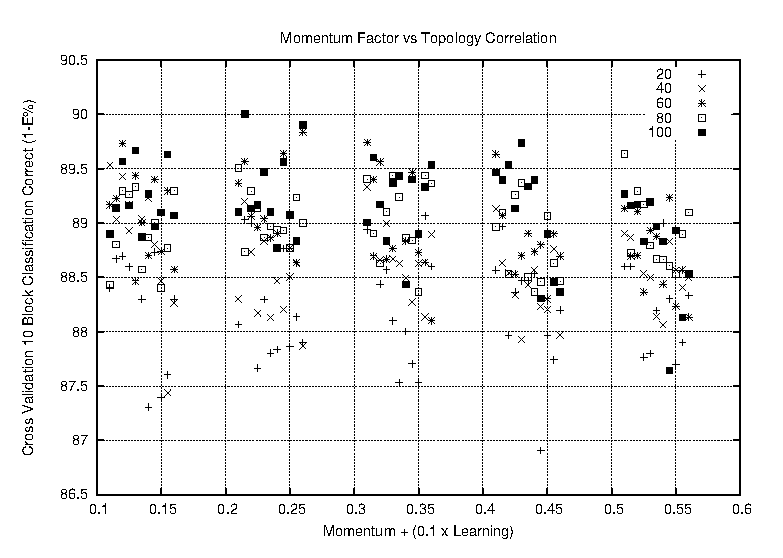
\includegraphics[]{momentum_topology.eps}
	}
	\caption[Terrain classification task: Correlation of the momentum factor over the topology]{Plot shows the neural network classification right classifications (1 - E\%) for the network topologies as a function of the training factors (Momentum+(0.Learning)) for the  terrain classification task. Each plotted point is obtained by performing a 10 block cross validation over the given normalized database.}
\end{figure}

\par Again we can see no real tendency of how the momentum factor affects the different topologies.

\subsubsection{Quick Propagation}

\par The same set of topologies where trained with the Quick propagation training algorithm in order to review if it could improve the Back propagation classification results.

\par An initial study training all topologies was launched in order to review the best topology for this Algorithm. For all experiments the learning factors where set to:
\begin{itemize}
	\item Learning: 0.3
	\item Max growth: 0.5
\end{itemize}


\par We can see in the previous graph that the one hidden layer neural network behave significantly better than the two hidden layer networks. Among the one hidden layer networks there is not a big difference in terms of correctly classified patterns but the neural network with 80 neurons seems to behave better; we will use this one for the in depth study of the learning parameters.

\par Once selected the best topology we performed a study of the quick propagation learning parameters by varying the learning parameter from 0.1 to 0.6 in 0.05 increments and for each learning factor value varying the maximum growth from 0.1 to 0.8 in 0.1 increments. 

\par The best result obtained was with a learning factor of 0.1 and a training factor of 0.7. 

\begin{table}[H] 
\caption{Test set comparison} %title of the table
\centering 
\begin{tabular}{c c} 
\hline\hline 
Cross validation & Oracle result \\
16.564 & 15.50 \\

\hline 
\end{tabular} 
\label{tab:dist_result} 
\end{table}



\subsubsection{Radial Networks}

\par For Radial Networks a different set of networks had to be created as the radial basis learning requires to have a radial function as the activation function of the hidden layer. 

\par In our study we created networks of: 20,40,60,80 \& 100 neurons on the hidden layer. For all of them the gaussian activation function was selected. 

\par Radial based training was significantly more complex to perform on the SNNS. A combination of three initialization functions had to be mixed up. Varying the default initialization or training parameter values from the ones explained in the SNNS manual caused the training algorithm to have numeric issues and not converge. Hence for this training algorithm only the topologies where varied.

\begin{figure}[H]
	\centerline{%
	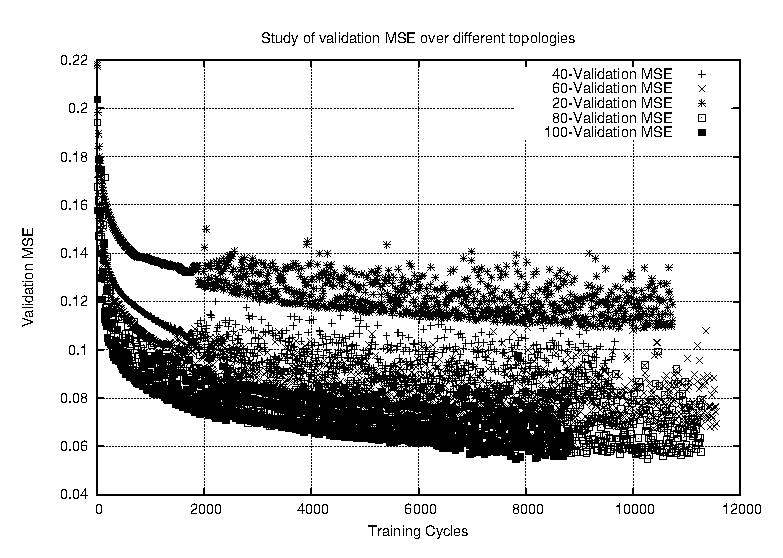
\includegraphics[]{validation_mse_rr.eps}
	}
	\caption[Terrain classification task: Topology study for radial networks - Validation MSE]{Plot shows the validation MSE for the radial network topologies as a function of the number of cycles trained for the  terrain classification task.}
\end{figure}

\par The above plot is not very clarifying but we can conclude that as we increase the number of neurons we are getting a better generalization of the validation set but it must also be noted that the algorithm does not present a convergence and hence the results obtained might not be very repeatable. 

\begin{figure}[H]
	\centerline{%
	\includegraphics[]{radial_topology.eps}
	}
	\caption[Terrain classification task: Topology study for radial networks - correct classification]{Plot shows the neural network classification right classifications (1 - E\%) for the radial network topologies as a function of the number of neurons on the hidden layer for the  terrain classification task. Each plotted point is obtained by performing a 10 block cross validation over the given normalized database.}
\end{figure}

\par As we have seen in the graph above the best neural network is of 100 neurons on the hidden layer but when sending the best trained network to the private test set oracle the best result was obtained with 40 neurons on the hidden layer. 

\section{Conclusions}

\par As we have seen in the previous tasks the best results have been obtained for the Radial based learning. The best results for each algorithm in the private test set has been as follows: 

\begin{table}[H] 
\caption{Private test set - best error results for training algorithms} %title of the table
\centering 
\begin{tabular}{c c c} 
\hline\hline 
Back-propagation & Quick-propagation & Radial Network \\
10.40 & 15.50 &  9.60 \\

\hline 
\end{tabular} 
\label{tab:dist_result} 
\end{table}

\par We have obtained the best results for Back-propagation and Radial based learning, being our radial network the network with least classification task in the board.

\par In future work it would be interesting to use the SVM software that has been integrated in the framework to study this task.  

\end{document}
